% Options for packages loaded elsewhere
\PassOptionsToPackage{unicode}{hyperref}
\PassOptionsToPackage{hyphens}{url}
%
\documentclass[
]{article}
\usepackage{amsmath,amssymb}
\usepackage{iftex}
\ifPDFTeX
  \usepackage[T1]{fontenc}
  \usepackage[utf8]{inputenc}
  \usepackage{textcomp} % provide euro and other symbols
\else % if luatex or xetex
  \usepackage{unicode-math} % this also loads fontspec
  \defaultfontfeatures{Scale=MatchLowercase}
  \defaultfontfeatures[\rmfamily]{Ligatures=TeX,Scale=1}
\fi
\usepackage{lmodern}
\ifPDFTeX\else
  % xetex/luatex font selection
\fi
% Use upquote if available, for straight quotes in verbatim environments
\IfFileExists{upquote.sty}{\usepackage{upquote}}{}
\IfFileExists{microtype.sty}{% use microtype if available
  \usepackage[]{microtype}
  \UseMicrotypeSet[protrusion]{basicmath} % disable protrusion for tt fonts
}{}
\makeatletter
\@ifundefined{KOMAClassName}{% if non-KOMA class
  \IfFileExists{parskip.sty}{%
    \usepackage{parskip}
  }{% else
    \setlength{\parindent}{0pt}
    \setlength{\parskip}{6pt plus 2pt minus 1pt}}
}{% if KOMA class
  \KOMAoptions{parskip=half}}
\makeatother
\usepackage{xcolor}
\usepackage[margin=1in]{geometry}
\usepackage{graphicx}
\makeatletter
\def\maxwidth{\ifdim\Gin@nat@width>\linewidth\linewidth\else\Gin@nat@width\fi}
\def\maxheight{\ifdim\Gin@nat@height>\textheight\textheight\else\Gin@nat@height\fi}
\makeatother
% Scale images if necessary, so that they will not overflow the page
% margins by default, and it is still possible to overwrite the defaults
% using explicit options in \includegraphics[width, height, ...]{}
\setkeys{Gin}{width=\maxwidth,height=\maxheight,keepaspectratio}
% Set default figure placement to htbp
\makeatletter
\def\fps@figure{htbp}
\makeatother
\setlength{\emergencystretch}{3em} % prevent overfull lines
\providecommand{\tightlist}{%
  \setlength{\itemsep}{0pt}\setlength{\parskip}{0pt}}
\setcounter{secnumdepth}{-\maxdimen} % remove section numbering
\ifLuaTeX
  \usepackage{selnolig}  % disable illegal ligatures
\fi
\IfFileExists{bookmark.sty}{\usepackage{bookmark}}{\usepackage{hyperref}}
\IfFileExists{xurl.sty}{\usepackage{xurl}}{} % add URL line breaks if available
\urlstyle{same}
\hypersetup{
  pdftitle={Sales Visualisation Project},
  pdfauthor={Dharmi Malde},
  hidelinks,
  pdfcreator={LaTeX via pandoc}}

\title{Sales Visualisation Project}
\author{Dharmi Malde}
\date{}

\begin{document}
\maketitle

\hypertarget{introduction}{%
\section{Introduction}\label{introduction}}

In the fast-moving world of retail, where what people like to buy can
change from season to season, it's really important for stores to
understand patterns, figure out insights, and use data to make smart
decisions.

In this data visualization project, we're going to understand how stores
sell things. We're going to look at how sales have changed over time and
look at the seasonal trend. We also going to look at the group of items
which gives maximum sales and look at what parameters have effect on
sales.

\hypertarget{data-discriptiobn}{%
\section{Data Discriptiobn}\label{data-discriptiobn}}

\hypertarget{sales-data-description}{%
\subsection{Sales Data Description:}\label{sales-data-description}}

\textbf{Date:} The date on which the sales data is recorded.\\
\textbf{Store\_nbr:} An identifier for the store where the products are
sold.\\
\textbf{Family:} The category or type of product sold (e.g., dairy,
snacks, beverages).\\
\textbf{Sales:} The total sales for a product family at a specific store
on a given date. Sales values may include fractional units (e.g., 1.5 kg
of cheese).\\
\textbf{Onpromotion:} The number of items in a product family that were
being promoted at a specific store on a given date.

\hypertarget{store-metadata}{%
\subsection{Store Metadata:}\label{store-metadata}}

\textbf{City:} The city where the store is located.\\
\textbf{State:} The state or region in Ecuador where the store is
situated.\\
\textbf{Type:} The type or format of the store (e.g., supermarket,
convenience store).\\
\textbf{Cluster:} A grouping of similar stores based on certain
characteristics.

\hypertarget{additional-data}{%
\subsection{Additional Data:}\label{additional-data}}

\textbf{Oil Price Data:} Daily oil price data, which is crucial due to
Ecuador's economic dependence on oil and its vulnerability to oil price
fluctuations.\\
\textbf{Holidays Data:} Information about holidays, which can impact
shopping patterns and sales.\\
\textbf{Daily Transaction Data:} Records of daily transactions for each
store, providing insights into customer behavior and sales trends.

This dataset provides a comprehensive view of sales at Favorita stores
in Ecuador, including details about products, stores, promotions, and
external factors like oil prices and holidays. Analyzing this data can
help identify sales trends, optimize inventory management, and make
data-informed decisions in the retail sector.

\hypertarget{exploratory-data-analysis}{%
\section{Exploratory Data Analysis}\label{exploratory-data-analysis}}

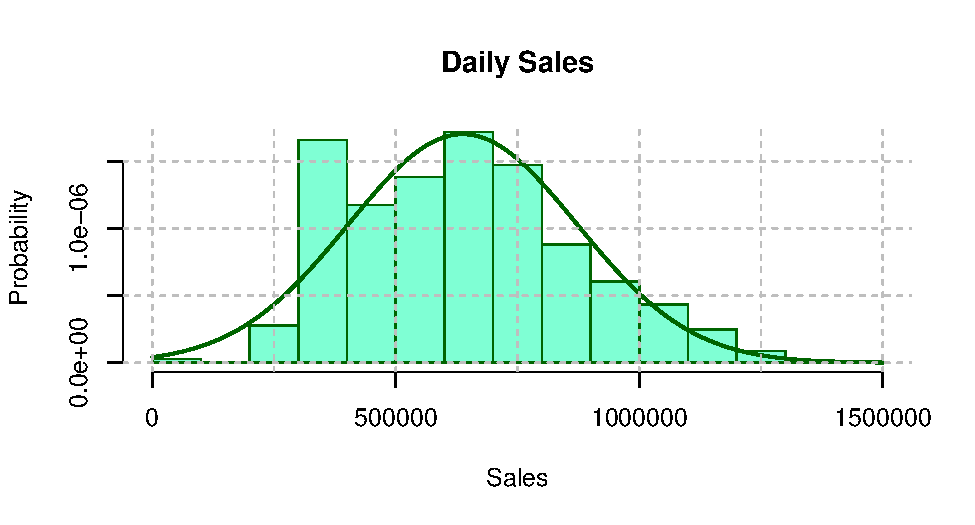
\includegraphics{Visualisation-Project_files/figure-latex/unnamed-chunk-1-1.pdf}
In the preceding visualization, our objective was to gain insights into
the daily sales patterns. The analysis of the graph reveals that the
data exhibits a central tendency, with the majority of daily sales
hovering around the 65,000 mark.

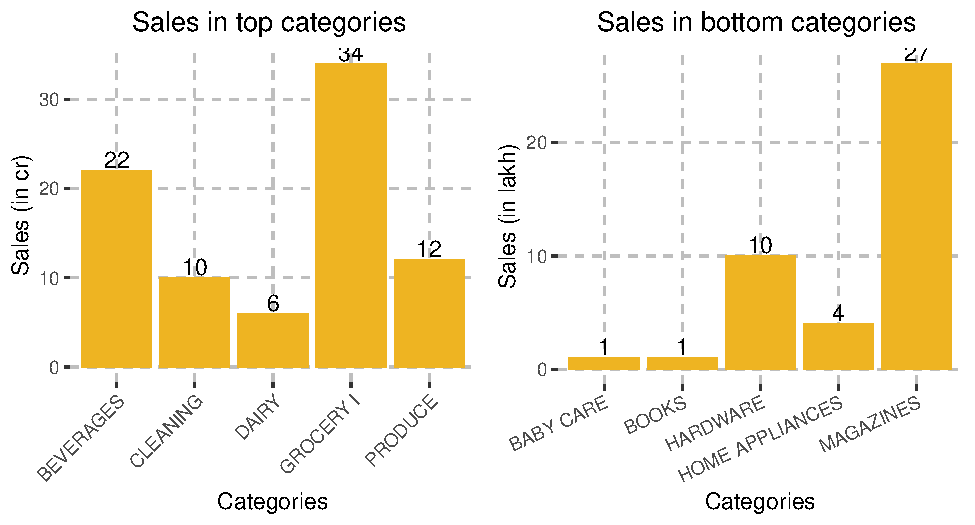
\includegraphics{Visualisation-Project_files/figure-latex/Ploting Family wise plot-1.pdf}
The preceding diagram provides valuable insights into the categorization
of items sold, distinguishing between the top and bottom categories.
Notably, the top category predominantly comprises daily-use items, while
the bottom category predominantly consists of occasional or infrequently
purchased items.

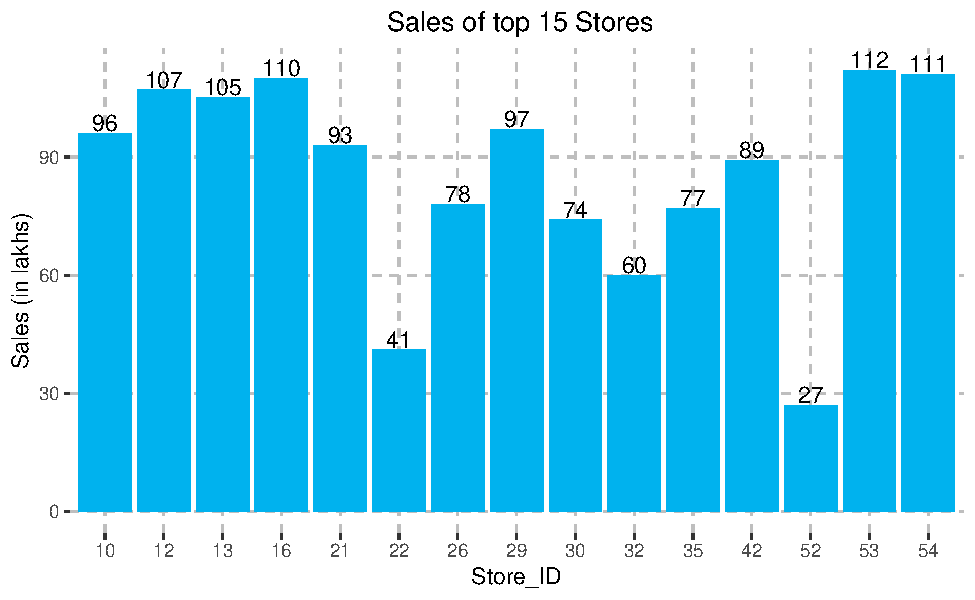
\includegraphics{Visualisation-Project_files/figure-latex/Plotting sales of top 15 stores-1.pdf}
The depicted diagram offers a glimpse into the sales performance of the
top 15 stores. Whereas the top 5 stores, identified by their store IDs
are 53, 54, 16, 12, and 13.

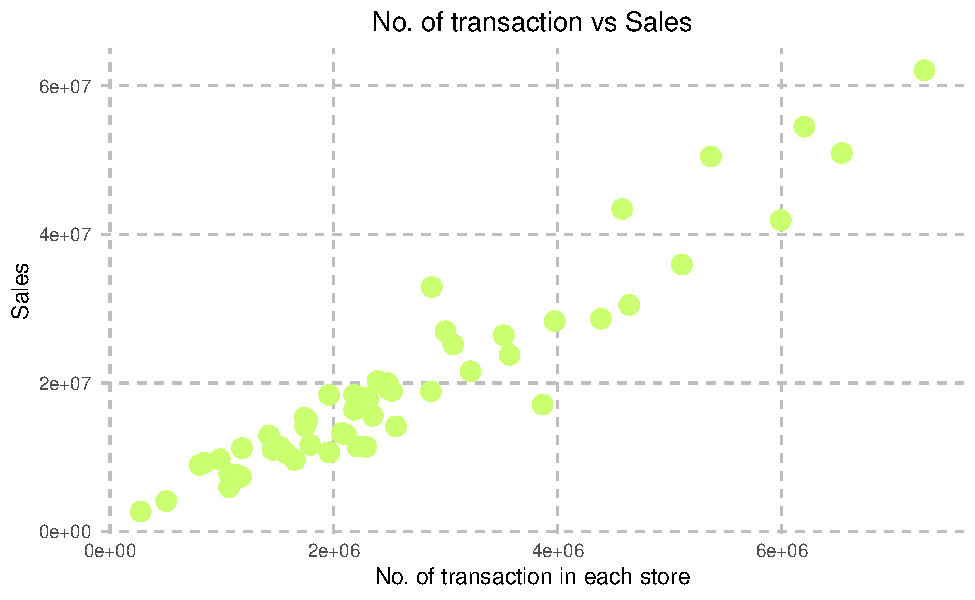
\includegraphics{Visualisation-Project_files/figure-latex/Transaction vs sales-1.pdf}
The scatter plot displayed above reveals a strong correlation between
the number of transactions and sales, suggesting that the average
transaction size across stores remains relatively consistent

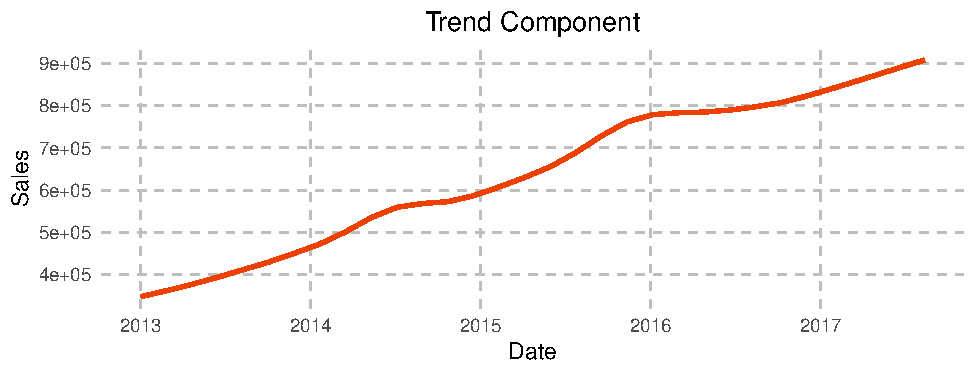
\includegraphics{Visualisation-Project_files/figure-latex/Time Series Decomposition-1.pdf}
The trend component plot above indicates a consistent upward trajectory
in sales over the years, signifying a notable increase in sales

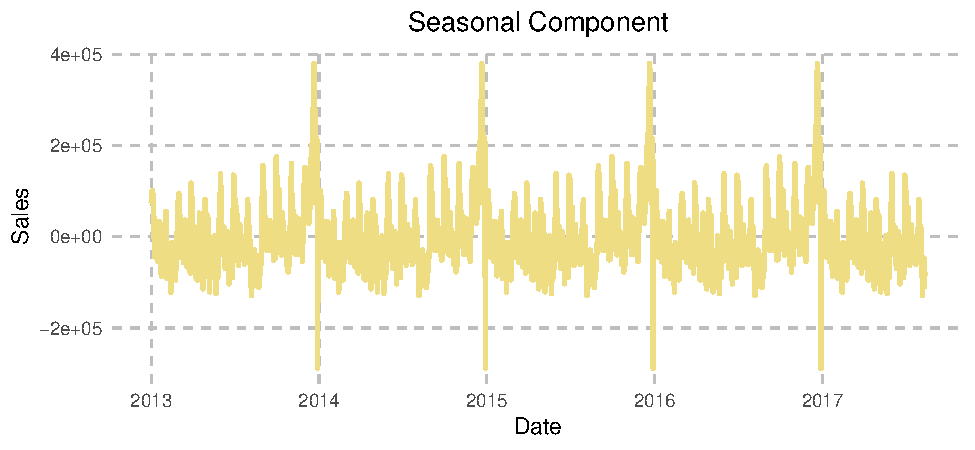
\includegraphics{Visualisation-Project_files/figure-latex/unnamed-chunk-2-1.pdf}
The seasonal component plot illustrates a noticeable spike in sales
leading up to Christmas, followed by a subsequent decline immediately
after the holiday period.

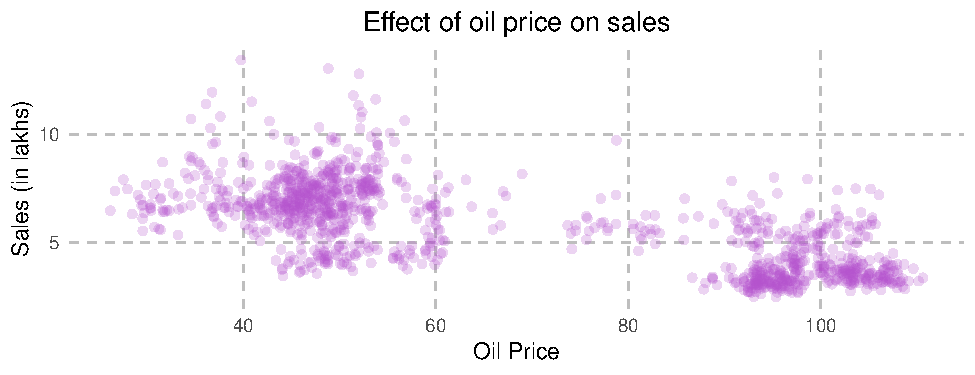
\includegraphics{Visualisation-Project_files/figure-latex/Effect of oil Price on sales-1.pdf}
The scatter plot presented above, depicting the relationship between oil
prices and sales, provides a clear inference. It suggests that when oil
prices exceed 75, there is a notable decrease in sales, whereas when oil
prices fall below this threshold, sales experience an uptick.

\hypertarget{results}{%
\section{Results}\label{results}}

\textbf{1. Daily Sales Patterns:} Our analysis of daily sales reveals a
distinct central tendency, with the majority of daily sales consistently
hovering around the 65,000 mark.

\textbf{2. Item Categorization:} Items sold fall into two discernible
categories. The top category predominantly includes essential daily-use
items, while the bottom category comprises occasional or infrequently
purchased items.

\textbf{3. Top-Performing Stores:} Within our dataset of the top 15
stores, we pinpoint five standout stores with IDs 53, 54, 16, 12, and
13, distinguished by their remarkable sales performance.

\textbf{4. Transaction-Sales Correlation:} A compelling observation
emerges from our scatter plot analysis, indicating a robust correlation
between transaction volume and sales. This suggests a consistent average
transaction size across stores.

\textbf{5. Sales Growth Over Years:} An unmistakable upward trend is
evident in our sales data over the years, signifying significant sales
growth.

\textbf{6. Seasonal Sales Dynamics:} Delving into the seasonal component
of our analysis, we observe a pronounced sales surge in the lead-up to
Christmas, followed by a post-holiday decline.

\textbf{7. Oil Price Influence:} Our exploration of the relationship
between oil prices and sales unveils a noteworthy insight. Sales exhibit
sensitivity to oil prices exceeding 75, with a significant drop observed
in such instances.

\hypertarget{conclusion}{%
\section{Conclusion}\label{conclusion}}

In conclusion, our data analysis and visualization provide valuable
insights into the dynamics of store sales. We observe a central tendency
in daily sales, significant categorization differences among items, and
the identification of top-performing stores. Additionally, we find a
strong correlation between the number of transactions and sales,
indicating consistent average transaction sizes.

Over the years, sales have demonstrated a positive trend, and there are
clear seasonal variations, with a surge in sales leading up to
Christmas. Notably, our analysis highlights the impact of oil prices on
sales, with sales showing sensitivity to oil prices exceeding 75.

These insights serve as a foundation for strategic decision-making,
allowing businesses to optimize their sales strategies, inventory
management, and promotional efforts. Understanding these patterns and
correlations can ultimately lead to enhanced sales performance and
profitability in the retail sector.

\end{document}
